\documentclass[french,a4paper]{article}
\setcounter{tocdepth}{4}
\setcounter{secnumdepth}{4}
\usepackage{graphicx}
\graphicspath{{img/}}
\title{PPII}
\usepackage[bottom=2.5cm,top=2.5cm,left=2.5cm,right=2.5cm]{geometry}
\author{Noé Steiner - Alexis Marcel - Lucas Laurent - Mathias Aurand-Augier}
\date{Octobre 2022}
\begin{document}

\maketitle
\newpage
\tableofcontents
\newpage
\section{Introduction}

Les enjeux climatiques n’ont jamais été aussi élevés. Notre planète arrive à la
fin de ses énergies fossiles. Les ressources deviennent rares, les changements
climatiques provoquent des pénuries, des sécheresses et des catastrophes
naturelles. Le mode de vie que nous connaissons aujourd’hui doit changer et
devenir plus écoresponsable. L’objectif est de changer les habitudes de
consommation de produits venants du monde entier en se restreignant à une zone
géographique bien plus petite. La politique actuelle serait de privilégier les
produits de notre pays mais essayons d’aller plus loin…

En effet, un mode de vie plus judicieux écologiquement serait de revenir à des
productions locales en passant directement par les producteurs. Certaines
personnes ont une surface de production( jardin, verger ) mais n’ont pas le
temps ou les moyens de s’en occuper. Tandis que d’autres personnes, n’ont pas
de terrain mais sont prêtes à donner de leur temps pour pouvoir consommer
localement.

Notre solution : utiliser les technologies modernes du web pour proposer une
application permettant à n’importe qui de créer/rejoindre un jardin mais
surtout de pouvoir gérer facilement un jardin sur lequel vont agir plusieurs
personnes.

\newpage
\section{Etat de l'art}

\newpage
\section{Gestion de projet}

\begin{figure}[h]
    \centering
    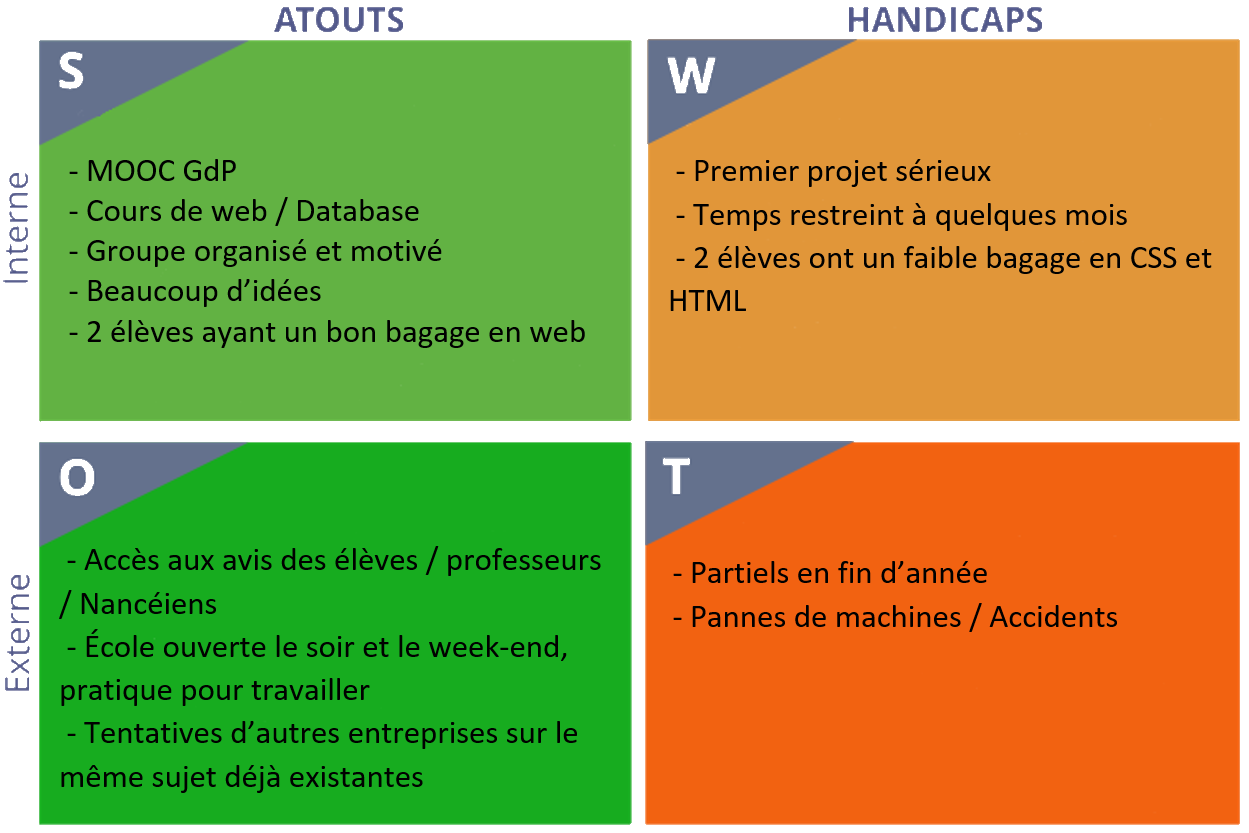
\includegraphics[width=0.75\textwidth]{img/SWOT.png}
    \caption{Analyse matricielle SWOT}
    \label{fig:mesh1}
\end{figure}

\begin{figure}[h]
    \centering
    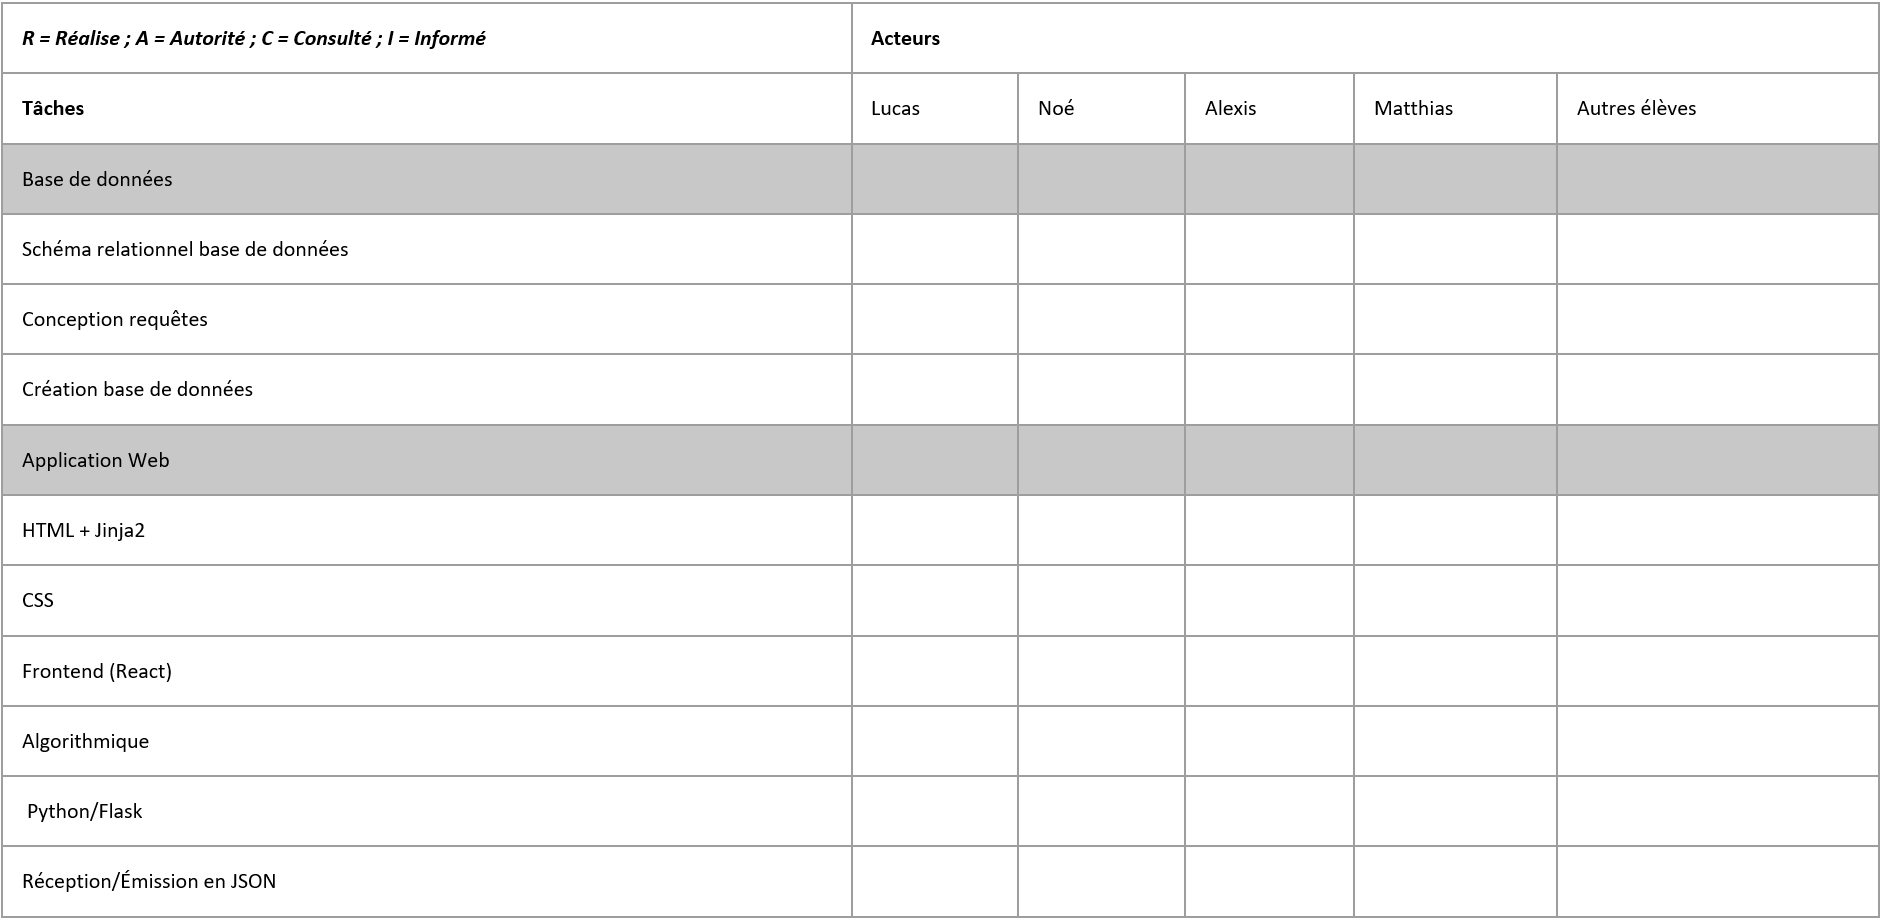
\includegraphics[width=0.75\textwidth]{img/RACI.png}
    \caption{Matrice RACI}
    \label{fig:mesh1}
\end{figure}

\begin{figure}[h]
    \centering
    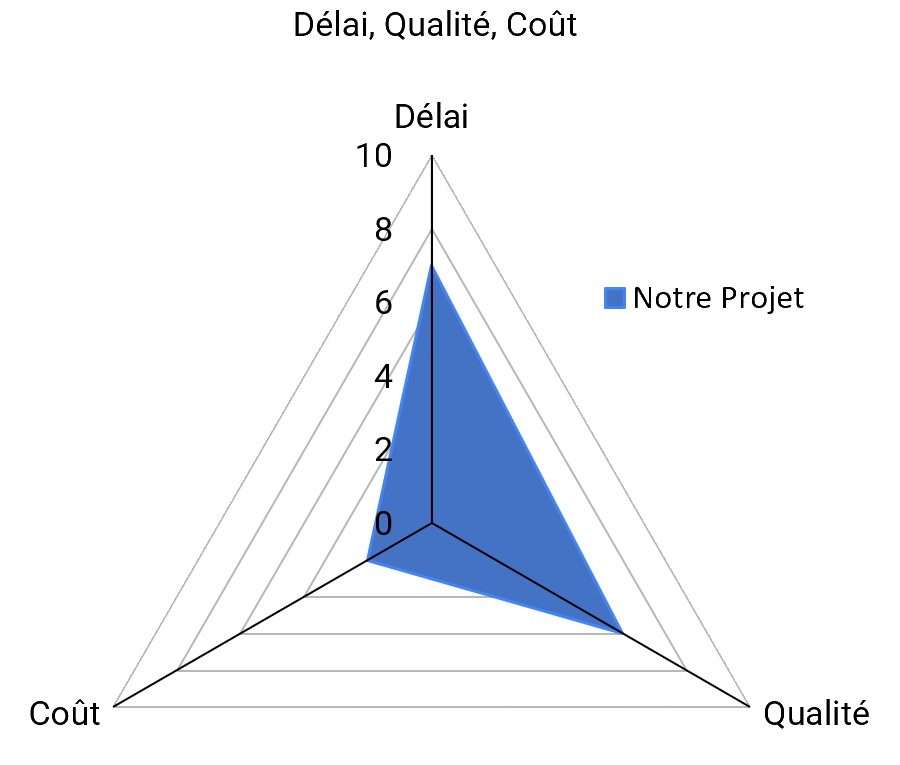
\includegraphics[width=0.75\textwidth]{img/triangle_QCD.png}
    \caption{Triangle CQD}
    \label{fig:mesh1}
\end{figure}

\begin{figure}[h]
    \centering
    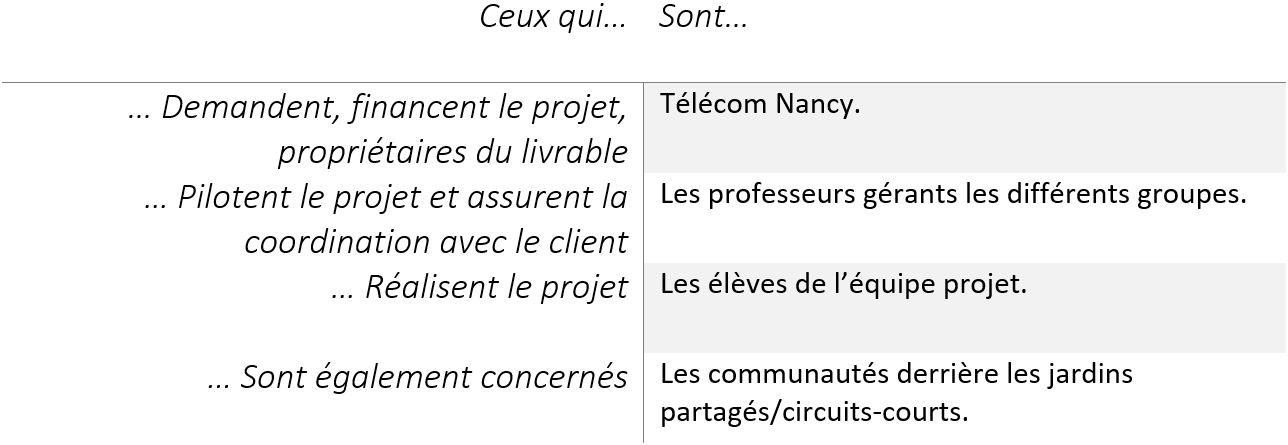
\includegraphics[width=0.75\textwidth]{img/parties_prenantes.png}
    \caption{Parties prenantes}
    \label{fig:mesh1}
\end{figure}

\begin{figure}[h]
    \centering
    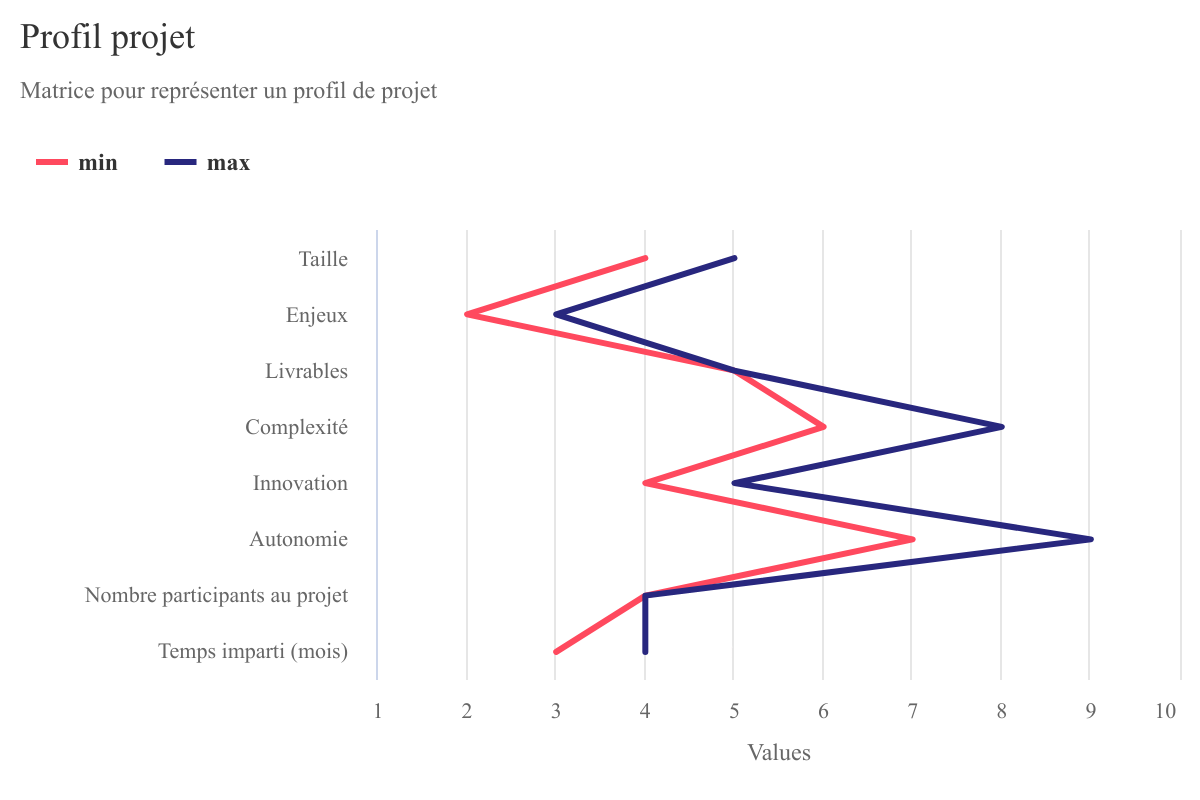
\includegraphics[width=0.75\textwidth]{img/profil_projet.png}
    \caption{Profil du projet}
    \label{fig:mesh1}
\end{figure}

\newpage
\section{Application proposée}
\subsection{Définitions}
\subsection{Application}
\subsection{Fonctionnalités principales}

Lorem ipsum dolor sit amet, consectetuer adipiscing elit. Etiam lobortis
facilisissem. Nullam nec mi et neque pharetra sollicitudin. Praesent imperdiet
mi necante...
\end{document}